\section{Downstream Analysis: \lme{}}
\label{sec:downstream}

To test whether write-time governance helps a long-horizon task, we evaluate a
stratified $180$-item slice of \lme{} ($6$ competencies $\times\,30$, seed $0$).
We report the completed homogeneous full-slice run (freeze \texttt{final-2.0},
denoted V12), then document why the earlier constructions on this track were
ineligible and are retained only as history. Throughout we use the exact ledger
labels --- \texttt{diagnostic\_only}, \texttt{failure\_replay\_only},
\texttt{incomplete}, and \texttt{final\_candidate} --- and do not collapse them
into a generic result.

\subsection{The homogeneous full-slice run}
\label{sec:downstream:final}

The V12 run evaluates all $180$ items with a single answer model
(\texttt{qwen/qwen3.5-9b}) and a single judge (\texttt{google/gemma-4-31b-it}),
with logged judge routing and \emph{zero} judge model fallbacks. On this run the
\ask{} controller reaches $137/180=76.1\%$ accuracy
(exact $95\%$ CI $70.0$--$82.2$), the highest of the five evaluated memory
systems and $12.8$ points above the strongest structural baseline (naive
overwrite, $114/180=63.3\%$). Answerable-only accuracy is $75.4\%$ over the
$171$ answerable items, and abstention accuracy is $88.9\%$ over the $9$
abstention items. The system ordering is monotone in memory sophistication
(Table~\ref{tab:lme}, Figure~\ref{fig:lme-accuracy}): no memory
($5.0\%$) $<$ recency ($23.9\%$) $<$ flat-vector retrieval ($44.4\%$) $<$ naive
overwrite ($63.3\%$) $<$ governed writes ($76.1\%$).

\begin{figure}[t]
\centering
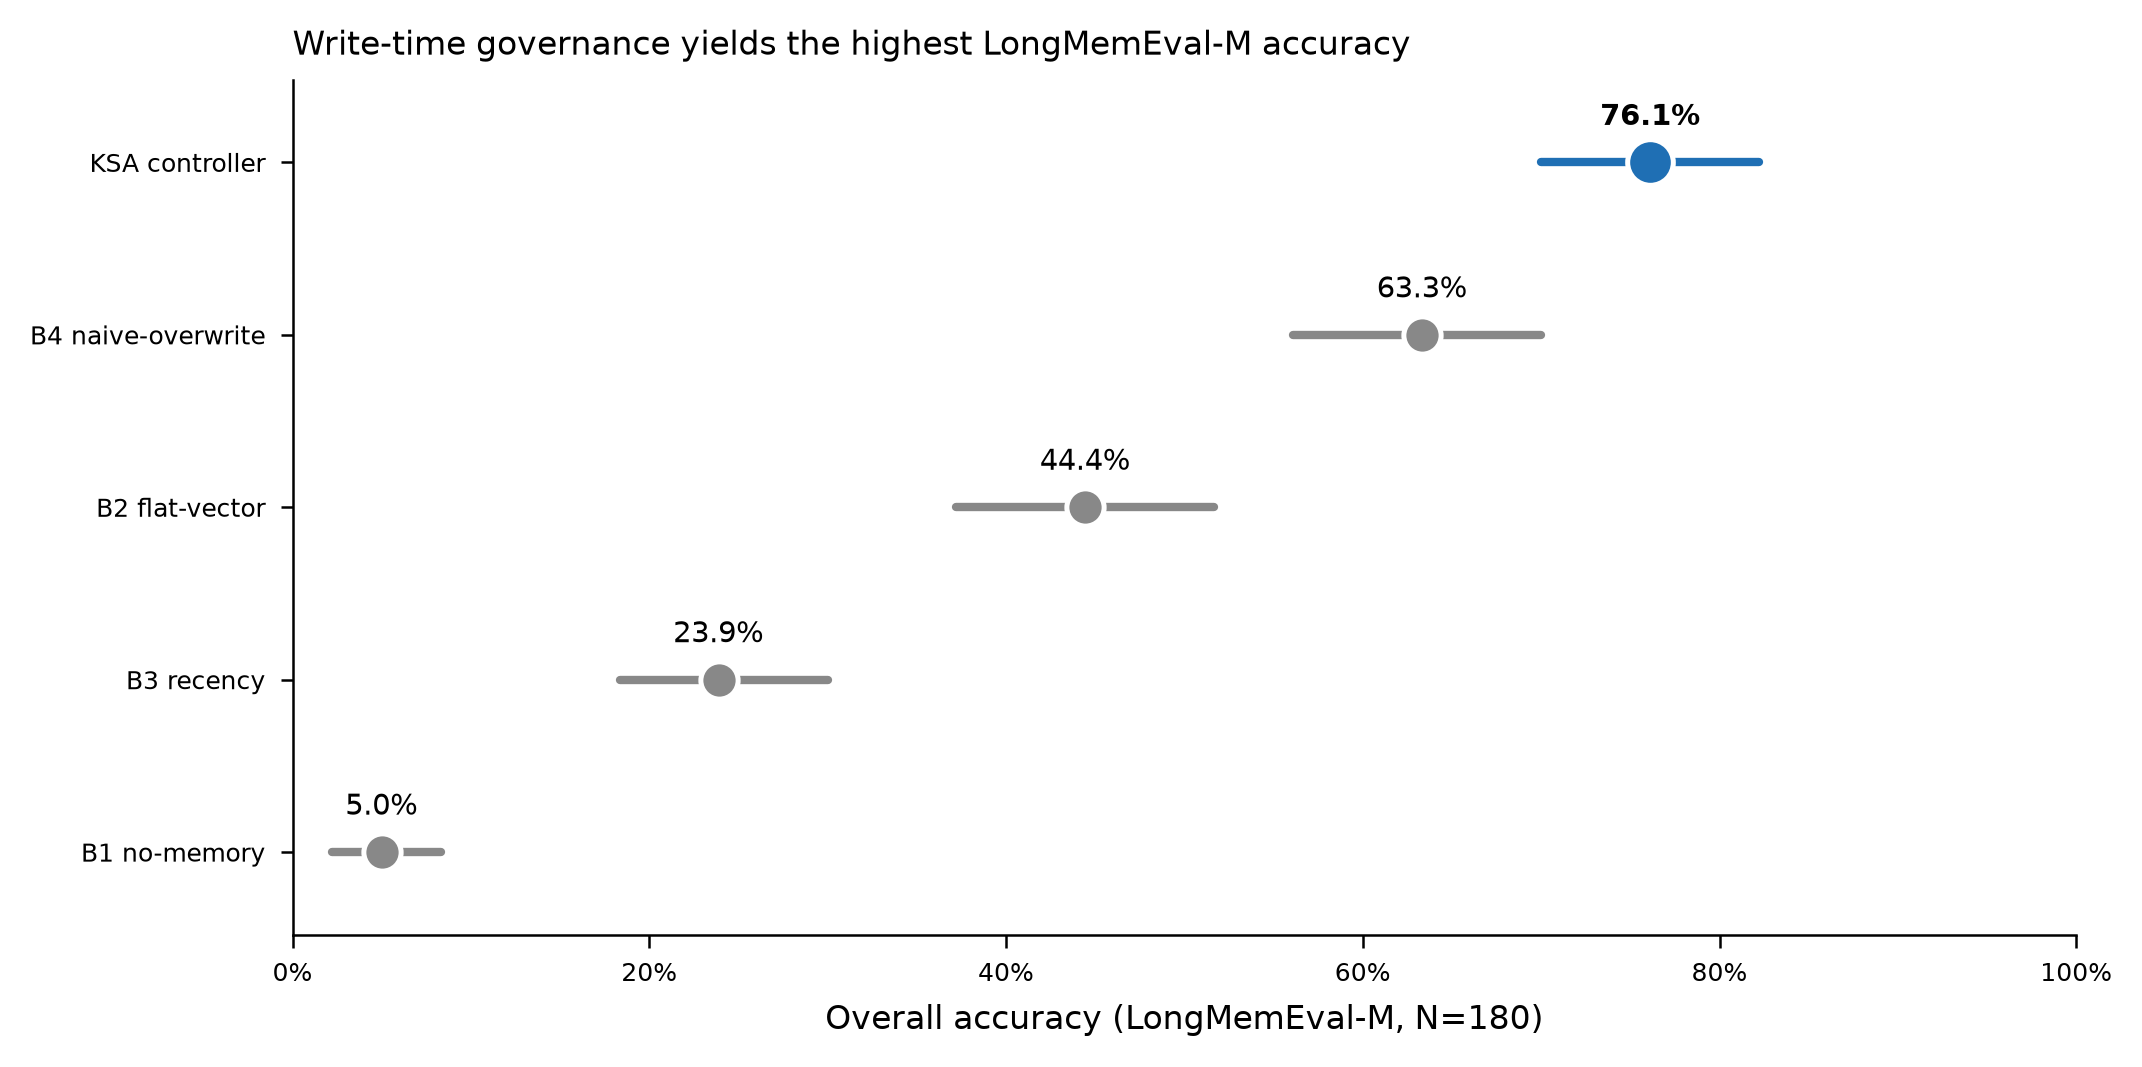
\includegraphics[width=\linewidth]{figures/lme_system_accuracy.png}
\caption{Overall \lme{} accuracy ($N=180$) for the five memory systems in the
homogeneous V12 run, with exact $95\%$ CIs. The \ask{} controller (highlighted)
leads all structural baselines.}
\label{fig:lme-accuracy}
\end{figure}

\begin{table}[t]
\centering
\small
\caption{\lme{} results. The V12 homogeneous full-slice run (freeze
\texttt{final-2.0}) is the eligible downstream result; earlier v7/v8 rows are
retained as history and remain ineligible per the ledger.}
\label{tab:lme}
\begin{tabular}{@{}l r r l@{}}
\toprule
Run or construction & correct/$n$ & accuracy & ledger status \\
\midrule
\multicolumn{4}{@{}l}{\emph{V12 homogeneous full-slice run (freeze final-2.0)}} \\
\quad B1 no-memory        & 9/180   & 0.0500 & \texttt{final\_candidate} \\
\quad B2 flat-vector      & 80/180  & 0.4444 & \texttt{final\_candidate} \\
\quad B3 recency          & 43/180  & 0.2389 & \texttt{final\_candidate} \\
\quad B4 naive-overwrite  & 114/180 & 0.6333 & \texttt{final\_candidate} \\
\quad \textbf{\ask{} controller} & \textbf{137/180} & \textbf{0.7611} & \texttt{final\_candidate} \\
\midrule
\multicolumn{4}{@{}l}{\emph{Earlier constructions (history; ineligible)}} \\
\quad v7 \ask{} controller     & 110/180 & 0.6111 & \texttt{diagnostic\_only} \\
\quad v8 replay of v7 failures & 25/70   & 0.3571 & \texttt{failure\_replay\_only} \\
\quad v8 carry-forward construction & 139/180 & 0.7722 & \texttt{failure\_replay\_only} \\
\quad v8 top-up of former successes & 71/84 & 0.8452 & \texttt{incomplete} \\
\bottomrule
\end{tabular}
\end{table}

Every item was scored by the single frozen judge: $40$ items were resolved by
deterministic guards (normalized match, no LLM call) and $140$ went to the LLM
judge, with $2$ scoring fallbacks logged. Nine items received a documented
semantic-equivalence adjudication that corrected judge scoring errors (for
example, accepting ``7 days'' as equivalent to ``1 week''); each carries a
written rationale and a preserved pre-adjudication backup of the machine
judgment.

Two provenance-bookkeeping items remain open on this run and do not affect any
reported number: the run's homogeneity gate flags a stale code/protocol hash for
the evaluation launcher, and the manifest was not written to a clean terminal
status after a resume. The per-system integrity checks (answer model, judge
routing, fallback counts) pass with empty error and warning lists.

\subsection{The contaminated v7 diagnostic}

The earlier v7 controller run is provider-contaminated: it accumulated $316$
HTTP-402 credit-exhaustion traces, $388$ empty-extraction fallbacks, at least
$12$ manual relaunches, and a no-op escalation tier (the ``big'' and ``fast''
models were identical). It is therefore \texttt{diagnostic\_only}, and on it
naive overwrite ($114/180$) edged the controller ($110/180$). The homogeneous
V12 run above supersedes that diagnostic and reverses the ordering under
controlled conditions.

\subsection{Why the 77.2\% construction was ineligible}

The v8 replay selected exactly the $70$ v7 controller failures and repaired
$25/70$. It was not a rerun of the full slice. The reported $139/180=77.2\%$
then combined $110$ carried-forward v7 successes ($108$ original
Gemma-judged successes plus two manual v7 adjudications), $25$ Qwen replay
repairs, and four later Codex/GPT-5 overrides. Before the four overrides, the
same construction was $135/180=75.0\%$. Judge identity and pipeline version are
therefore confounded with whether an item had previously failed, and the fixes
were evaluated on the failures that motivated them. The ledger correctly labels
both figures \texttt{failure\_replay\_only}, not final or diagnostic full-run
accuracy.

The top-up is non-empty and directly contradicts the carry-forward assumption.
It re-executed $84/110$ former v7 successes under the v8 attempt: $71$ remained
correct and $13$ regressed. Combining those $71$ with the $25$ raw replay
repairs gives $96/154$ observed. Treating the $26$ unresolved items as all wrong
or all correct gives full-slice raw bounds of $53.3$--$67.8\%$. Retaining the
four replay overrides gives bounds of $55.6$--$70.0\%$. Even the optimistic
bound is below $77.2\%$, so this attempt cannot reproduce the carry-forward
construction. These are missing-data bounds, not confidence intervals.

\subsection{Single-session preference: carry-forward artifact and taxonomy}

Single-session preference (SSP) was the weakest v7 competency at $11/30$. That
is a contaminated diagnostic run only, not a clean v8 measurement.
The replay targeted the $19$ v7 SSP failures and repaired $0/19$; the top-up
completed $10/11$ former SSP successes and retained only $8/10$. Across the two
selected subsets, $8/29$ completed SSP items are correct and one is unresolved,
so the maximum is $9/30$. The earlier statement that SSP stayed ``unchanged at
$11/30$'' is only a carry-forward artifact.

The replay and v7 prompt contexts differ, so persistence of the $19$ failures
does \emph{not} isolate the answer model or support a same-context causal claim.
It does, however, identify a concrete set for descriptive error analysis. By
inspecting whether each decisive gold fact appeared in the constructed prompt,
we classified the $19$ v7 failures as shown in Table~\ref{tab:ssp}.
Grounding-supply failures (retrieval omission plus cross-session contamination)
are primary in $10/19$ and present in $15/19$; answer-side failures are primary
in $9/19$. This taxonomy describes the inspected artifacts and does not prove
that the write policy is causally exonerated.

\begin{table}[t]
\centering
\small
\caption{Primary-category taxonomy of the $19$ v7 SSP failures, from the
released taxonomy artifact.}
\label{tab:ssp}
\begin{tabular}{@{}l r r@{}}
\toprule
Primary failure category & Count & Share \\
\midrule
retrieval-omission                         & 6 & 31.6\% \\
cross-session-contamination                & 4 & 21.1\% \\
target-attribute-extraction-miss           & 3 & 15.8\% \\
distractor-entity-binding                  & 2 & 10.5\% \\
polarity-error                             & 2 & 10.5\% \\
unsupported-answer-specificity             & 1 & 5.3\% \\
immediate-request-vs-enduring-preference   & 1 & 5.3\% \\
\midrule
\multicolumn{3}{@{}l}{\emph{Grounding-supply family: primary $10/19$, present $15/19$}} \\
\multicolumn{3}{@{}l}{\emph{Answer-side family: primary $9/19$}} \\
\bottomrule
\end{tabular}
\end{table}

\subsection{Proposed intervention and remaining headroom}

The taxonomy motivates a proposed but unexecuted intervention: represent each
preference as a typed record (holder/target/attribute/polarity/scope/stability/
source), require retrieval to surface the supporting-session record for the
query subject, and constrain answers to retrieved, grounded preferences while
honoring explicit negatives. We make no accuracy claim for this design. It is
directed at the competency where the V12 controller has the most headroom:
single-session-preference remains its weakest competency at $53.3\%$, alongside
multi-session and temporal-reasoning at $63.3\%$ each, whereas knowledge-update
and single-session-assistant are effectively solved at $96.7\%$
(Figure~\ref{fig:lme-competency}).

\begin{figure}[t]
\centering
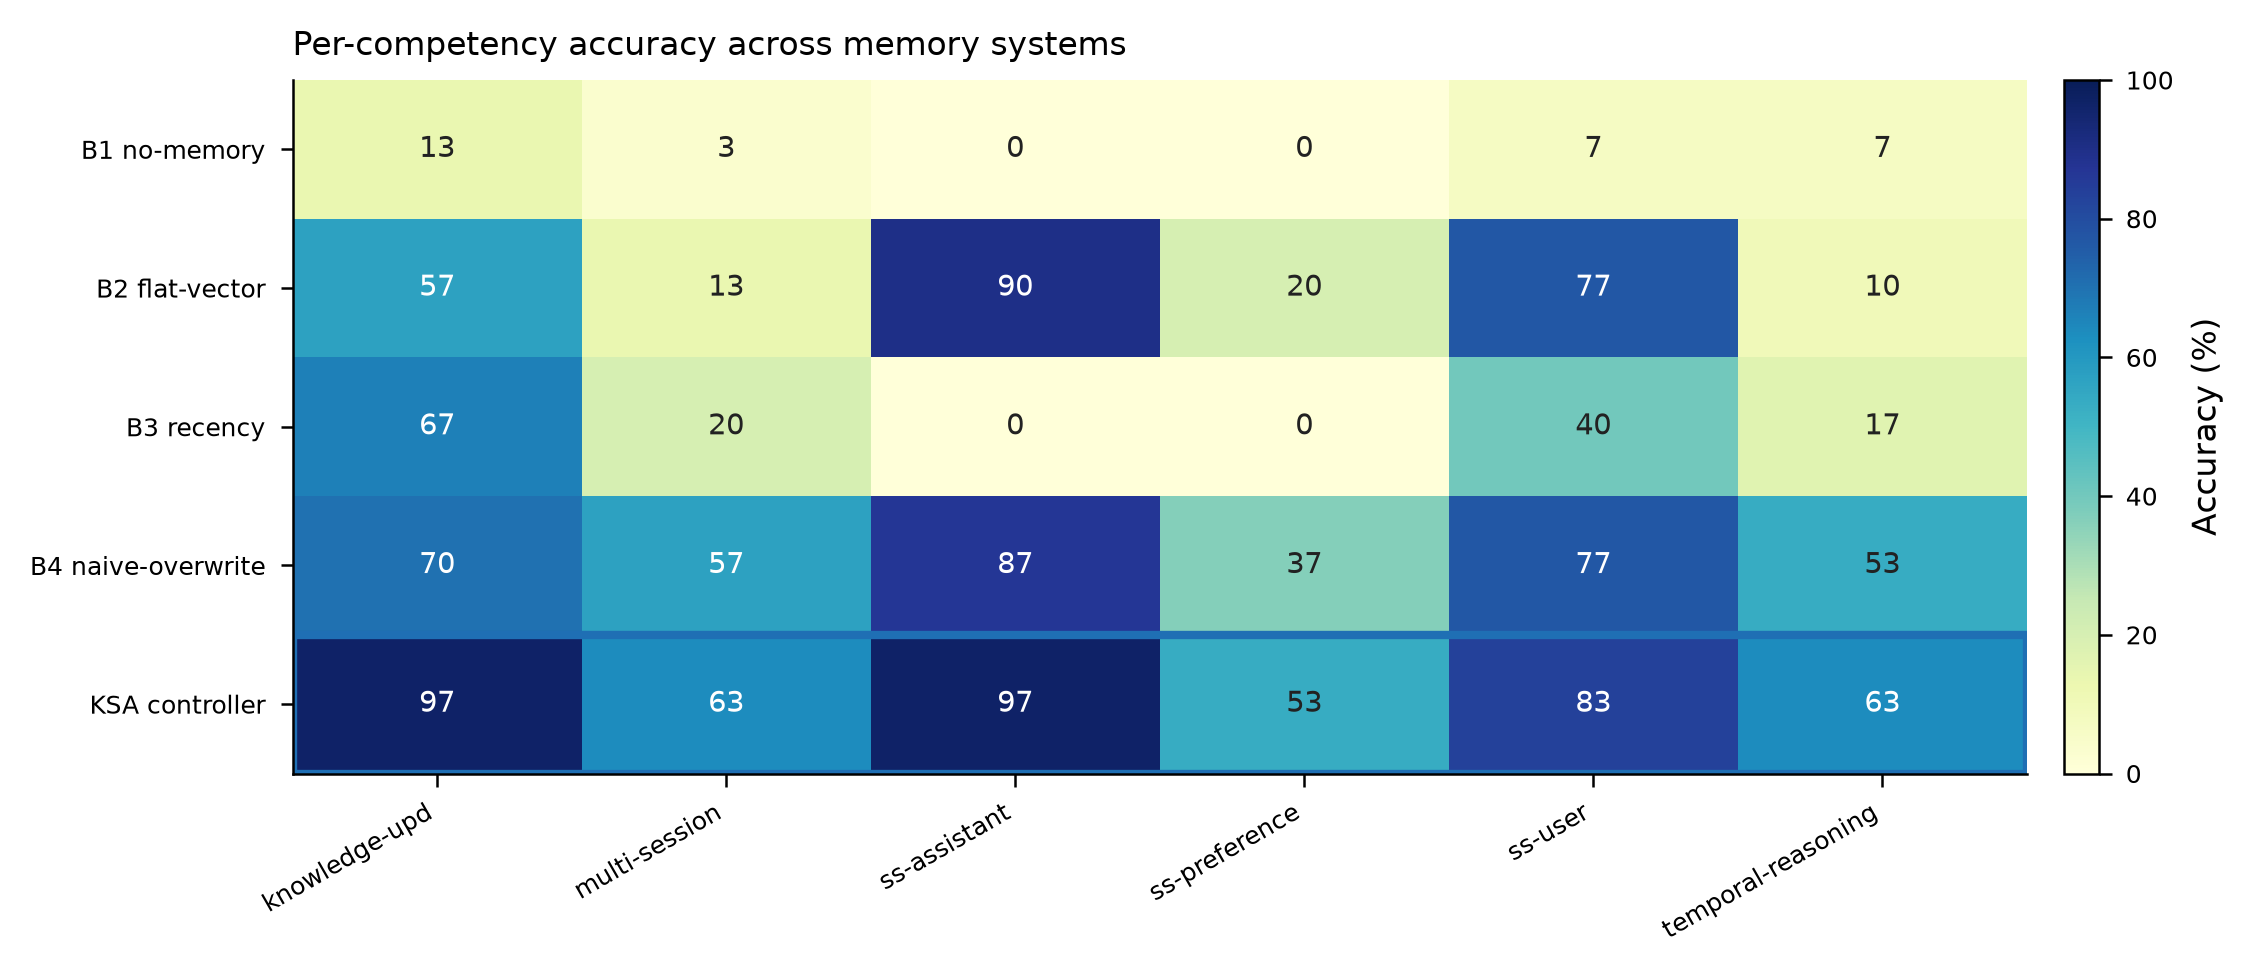
\includegraphics[width=\linewidth]{figures/lme_competency_heatmap.png}
\caption{Per-competency accuracy across the five memory systems in the V12 run.
The \ask{} controller (outlined row) leads or ties on every competency; its
remaining headroom is concentrated in preference and reasoning-heavy
competencies.}
\label{fig:lme-competency}
\end{figure}

The homogeneous full-slice run described in
Section~\ref{sec:downstream:final} is the eligible downstream result. It
evaluates all $180$ items with one answer model and logged judge routing under
the frozen final protocol. The experiment registry moves this run from
\texttt{externally\_pending} to \texttt{final\_candidate} with the controller at
$76.1\%$; promotion to \texttt{final} in the canonical results ledger is pending
the two open provenance-bookkeeping items (stale launcher hash, non-finalized
manifest status), which are tracked separately and do not enter the reported
score.
